%%%%%%%%%%%%%%%%%%%%%%%%%%%%%%%%%%%%%%%%%%%%%%%%%%%%%%%%%%%%%%%%%%%%%%%%%%%%%%%
%
% 
% 
%%%%%%%%%%%%%%%%%%%%%%%%%%%%%%%%%%%%%%%%%%%%%%%%%%%%%%%%%%%%%%%%%%%%%%%%%%%%%%%


\chapter{Simulation Method}
\label{sec:Simulation Method}

\section{FEM}


\section{Simulation Setup}
\subsection{Sphere vs Rigid Plane}
In this simulation the collision of two viscoelastic spheres is studied. Both the spheres have the same magnitude of velocity but opposite directions. Therefore to simplify the model and computation, instead of simulation two spheres colliding, a single sphere colliding against a rigid plane can be simulated. This setup would be equivalent to the original problem as both the spheres are the same in all aspects except for having different directions of velocities.

\subsection{Symmetry}
To further simplify the model, instead of considering the complete sphere, only a 2D semi-circular cross-section is considered. As the spheres are symmetric about the central rotational axis and the angle of contact is 90 degrees, there would not be any velocity in the Y direction. 

\subsection{Mesh}

\begin{figure}
    \centering
	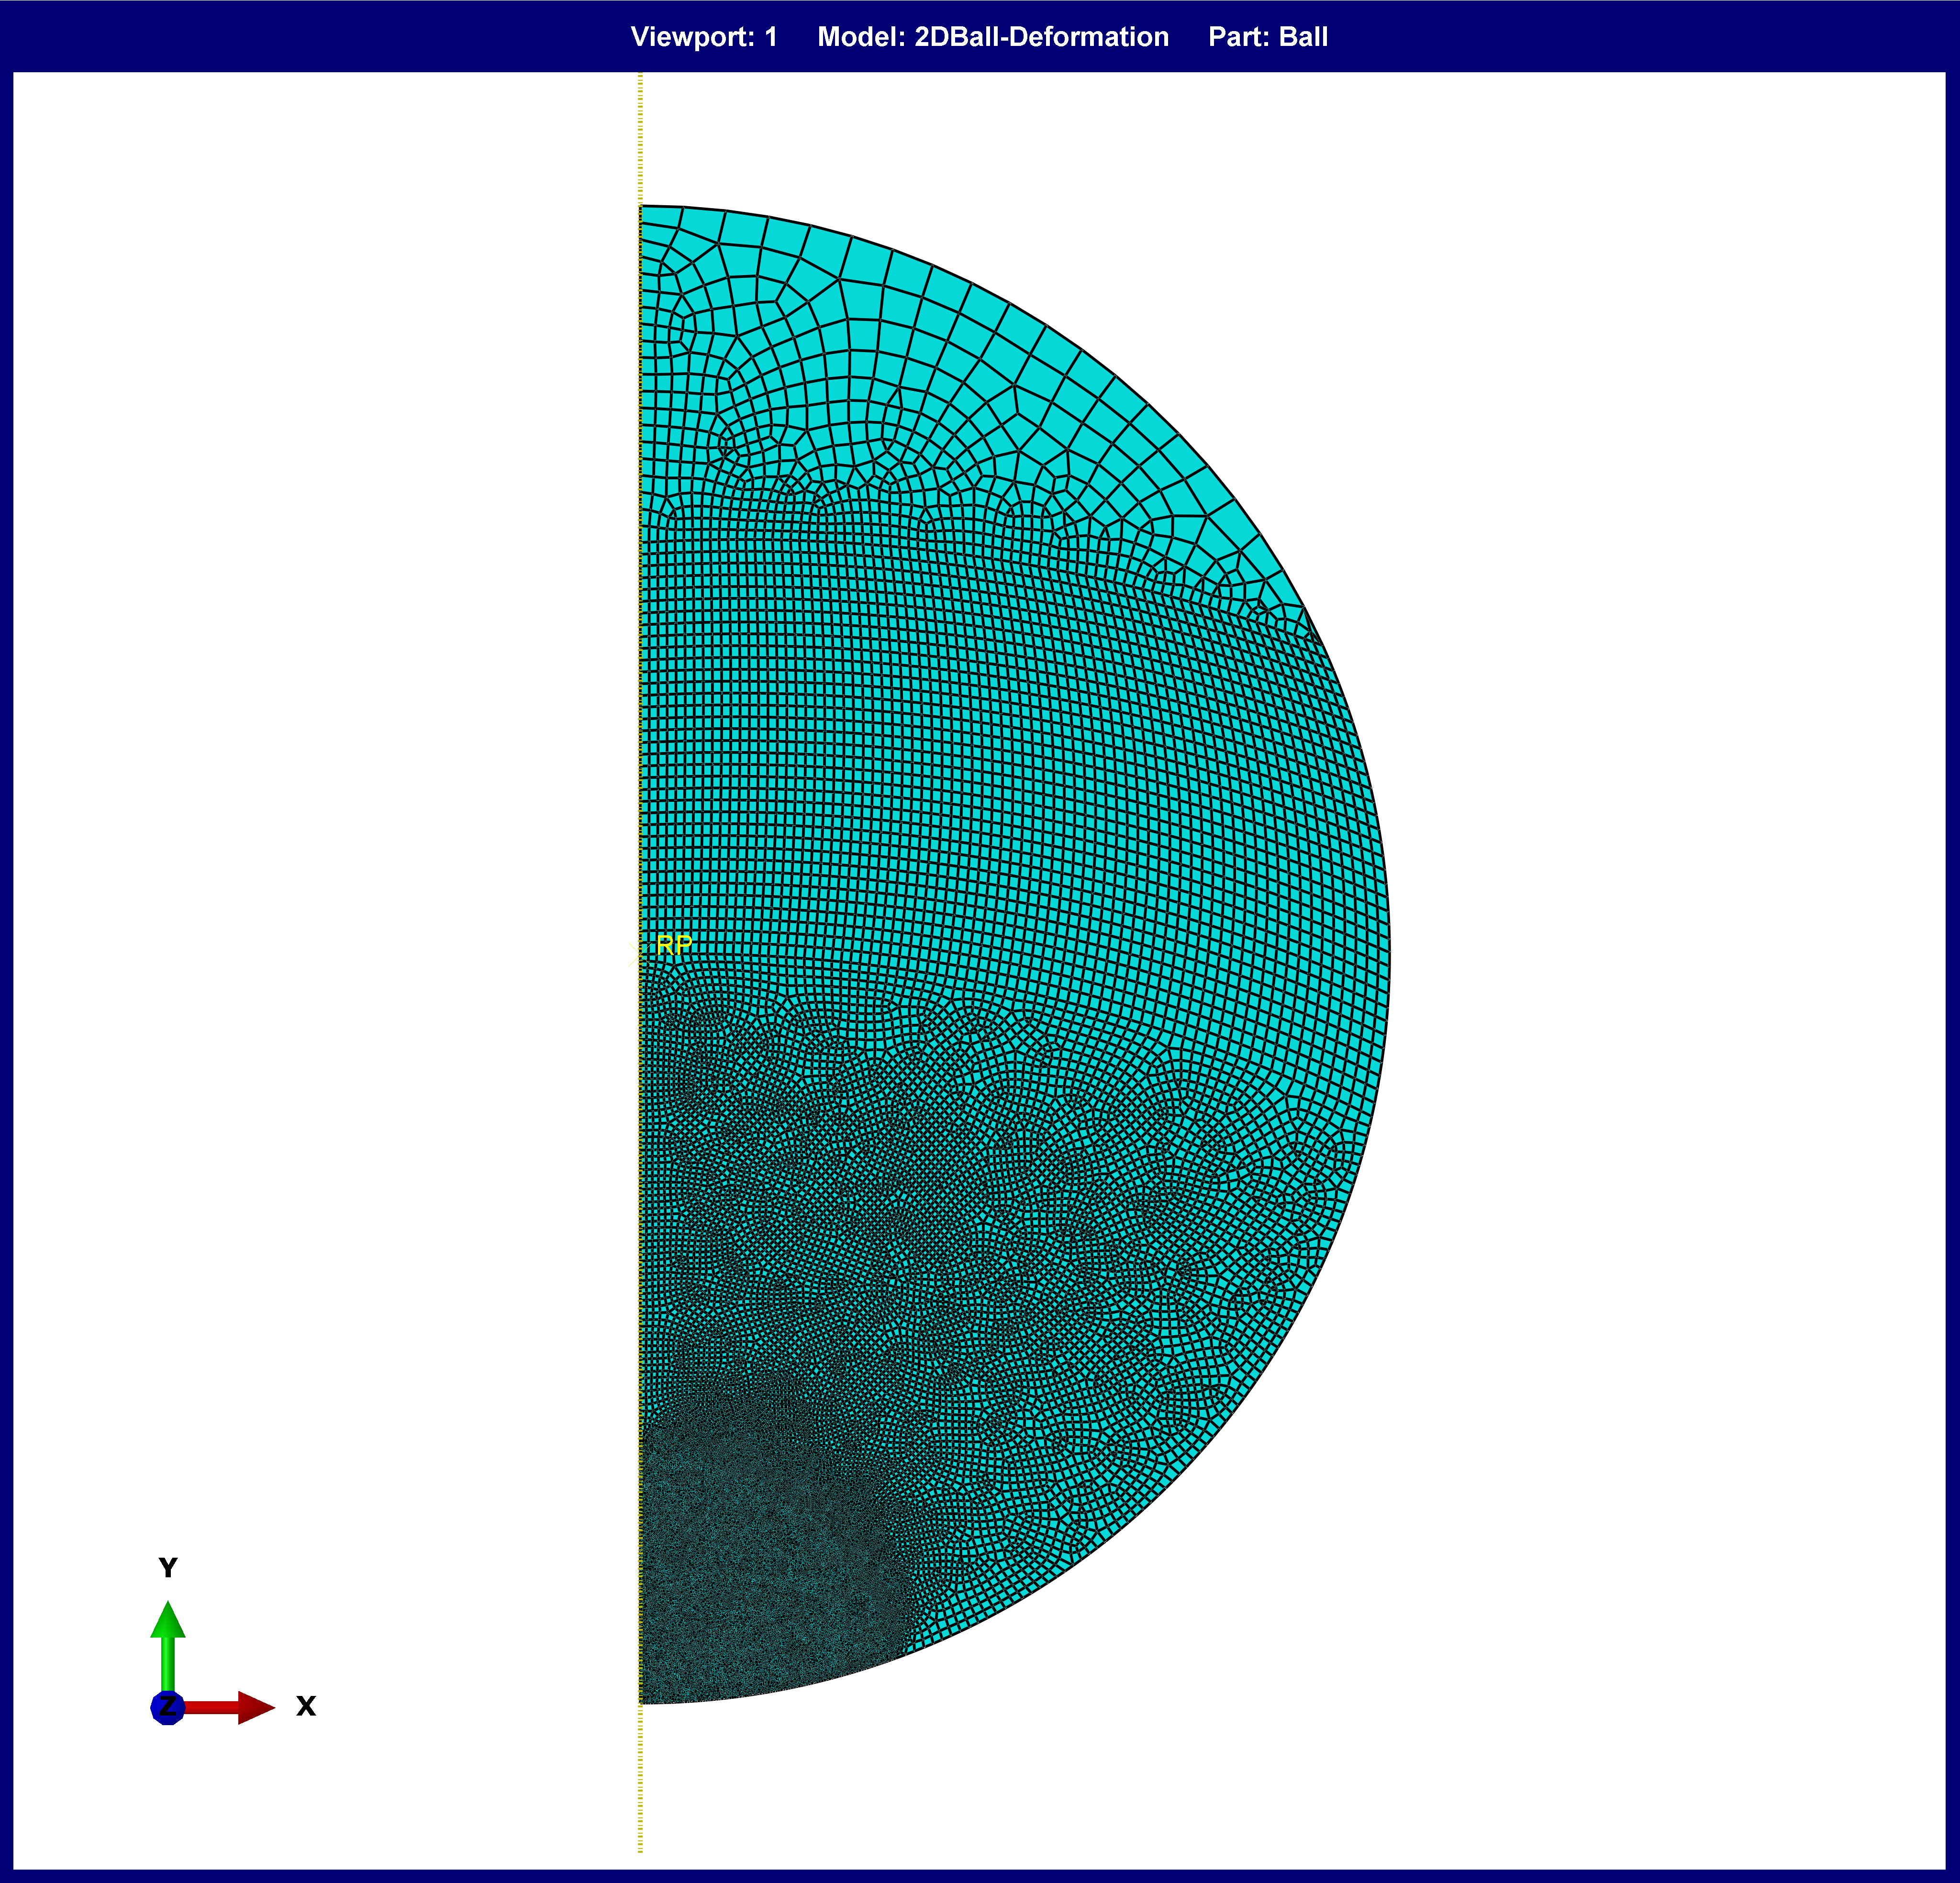
\includegraphics[scale=0.075]{../images/Mesh/Mesh.png}
	\caption{Mesh}
	\label{fig:mesh}
\end{figure}

The \ref{fig:mesh} shows the mesh used in the simulation. We can see that the mesh is finer at the bottom of the sphere as it is the point of contact and would undergo massive deformation during the impact. 

\begin{figure}
    \centering
	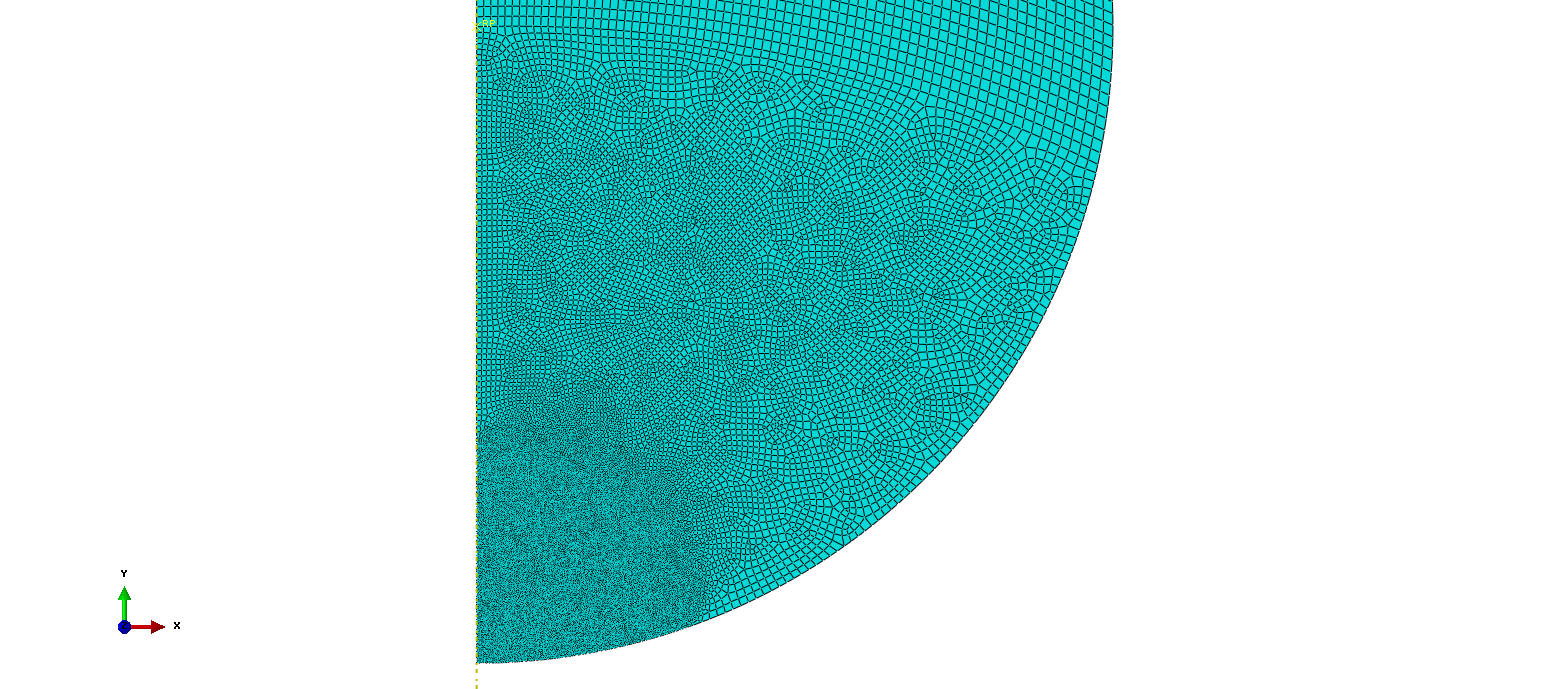
\includegraphics[scale=0.075]{../images/Mesh/Mesh_Bottom_Half_lowRes.png}
	\caption{Bottom Half of Mesh}
	\label{fig:mesh_bottom_half}
\end{figure}

The \ref{fig:mesh_bottom_half} shows an enlarged image of the bottom half of the mesh. We can see the degree of fineness of the mesh compared to the other half of the sphere.


\subsection{Rigid Plane}

The figure shows the rigid plane against which the sphere would be colliding. 

\section{Measurement Quantities}

\subsection{Deformation of Center of Mass}

\subsection{Kinetic Energy}

\subsection{Strain Energy}

\subsection{Co-efficient of Restitution}

The co-efficient of restitution describes the energy transfer 	 

\section{Verification}
